\section{Общее представление о системе}
\pretolerance10000

FreeHackQuest -- это платформа для обучения, проведения практических занятий и соревнований по компьютерной безопасности в формате тестирования на проникновение внутри среды, моделирующей работу информационной инфраструктуры организации. FHQ включает в себя учебник, различные задачи для решения, связанные с администрированием, криптографией, компьютерно-криминалистической экспертизой, стеганографией и многими другими направлениями информационной безопасности.\par
FreeHackQuest представляет собой клиент–серверную многофункциональную систему с подсистемами и состоит из следующих основных компонентов:
\begin{itemize}
\item сервер -- отвечает за обработку запросов со стороны клиента;
\item LXD (сервер виртуальных машин) -- предназначен для размещения контейнеров, необходимых, для изолированного выполнения сервисов с уязвимостями;
\item MySQL (сервер баз данных) -- отвечает за хранение и предоставление информации;
\item клиент -- отвечает за формирование запросов подсистеме сервера и представление ответов со стороны сервера;
\item административный клиент -- отвечает за управление системой.\par
\end{itemize}
\vspace{\baselineskip}

Структура системы представлена на рисунке 2.
\begin{center}
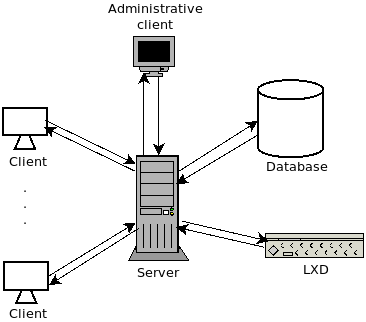
\includegraphics[width=0.65\textwidth]{1}\\
Рисунок 2 -- Структура системы\\
\end{center}
\vspace{\baselineskip}

\subsection{Описание стека технологий системы}
Архитектура клиент-сервер определяет лишь общие принципы взаимодействия между компьютерами, детали взаимодействия определяют различные протоколы. Данная концепция нам говорит, что нужно разделять машины в сети на клиентские, которые делают запрос, и на серверные, которые отвечают на него. При этом взаимодействие всегда начинает клиент, а правила, по которым происходит взаимодействие описывает протокол.\par
За взаимодействие между сервером и клиентами, в том числе с административным клиентом, отвечает протокол WebSocket (WS/WSS). Данный протокол связи поверх TCP-соединения предназначен для обмена сообщениями между браузером и веб-сервером в режиме реального времени.\par
MySQL как СУБД, если рассматривать её в рамках клиент-серверной архитектуры, является прежде всего программой-сервером, который может получать от различных клиентов, задачи по работе с данными (посредством SQL-запросов).\par 
Этими клиентами могут быть:
\begin{itemize}
\item собственная-программа клиент работающая в командной строке;
\item скрипт, написанный на каком-нибудь языке программирования, например, на PHP (так называемый <<запрос из приложения>>);
\item программа для работы с данными в графическом интерфейсе.\par
\end{itemize}
\vspace{\baselineskip}

Взаимодействие c e-mail осуществляется посредством SMTP-протокола -- протокола для исходящей связи по электронной почте. Простой протокол передачи почты (SMTP), используется для связи с удаленным сервером и последующей отправки сообщений с локального клиента на удаленный сервер, и в конечном итоге на сервер получателя сообщений. SMTP используется исключительно для отправки сообщений.\par
Если выполняется условие if enabled lxd, то сервер обращается к серверу виртуальных машин (LXD).\par
\vspace{\baselineskip}

\subsection{LXD}
Система виртуализации необходима для изолированного выполнения сервисов с уязвимостями, так как участники могут скомпрометировать машину, на которой развернута моделируемая инфраструктура организации. Система виртуализации должна обладать сетевым управлением, такое требование позволяет размещать контейнеры на отдельной от backend сервера машине. Например, у хостинг-провайдеров можно арендовать необходимые вычислительные мощности на время проведения практики и обучения.\par
В качестве системы виртуализации выбран LXD (LXC). LXD это то, что называется легковизор. Ядром LXD является демон, который предлагает API REST для управления контейнерами подобно виртуальным машинам. Чтобы создавать, управлять и мониторить множество уязвимых сервисов с определенными настройками сети прямо в административной странице FreeHackQuest, появилась необходимость интеграции FreeHackQuest с LXD.\par
Система оркестрации, предназначенная для развертывания сервисов с уязвимостями и запуска ботов, имитирующих поведение пользователей позволяет отправлять HTTP GET, POST, PUT, DELETE запросы серверу LXD, а также создавать, получать, запускать, останавливать и удалять контейнеры, узнавать информацию о контейнере.\par
Система оркестрации является частью подсистемы сервера FreeHackQuest и имеет структуру взаимодействия, показанную на рисунке 3.\par
\begin{center}
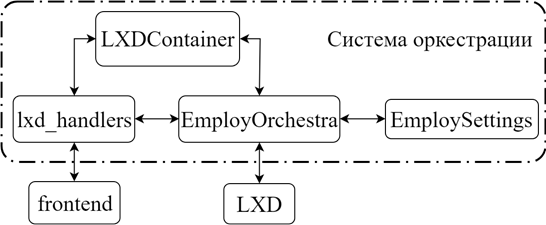
\includegraphics[width=0.65\textwidth]{2}\\
Рисунок 3 -- Структура взаимодействия системы оркестрации\\
\end{center}
\vspace{\baselineskip}
\clearpage